\section{Timing}\label{sec:timing}
\subsection{Profiling}
In order to find the bottlenecks of our simulators, we first profiled our code
using Intel's VTune Amplifier, as shown in \figref{amplxe-command}.

\begin{figure}[h]
\footnotesize
\begin{verbatim}
amplxe-cl -collect advanced-hotspots ./shallow
amplxe-cl -report hotspots -source-object function=<NAME>

amplxe-cl -report hotspots -r r001ah/ > all
amplxe-cl -report hotspots -source-object function="Central2D
<Shallow2D, MinMod<float>>::compute_step" > compute_step
\end{verbatim}
\caption{VTune Amplifier Command}
\label{fig:amplxe-command}
\end{figure}

\subsection{Initial Profile Result}

From \figref{initial-profile-result}, we concluded that \ttt{limited\_derivs},
\ttt{compute\_step}, and \ttt{compute\_fg\_speeds} take the longest time (see
\ttt{profile.sh} for more information). Among these results, the
\ttt{limited\_derivs} function was the worst bottleneck.

\begin{figure}[h]
\footnotesize
\begin{verbatim}
Function                     Module        CPU Time
-----------------------------------------  --------
limited_derivs               shallow         1.378s
compute_step                 shallow         0.640s
compute_fg_speeds            shallow         0.219s
_IO_fwrite                   libc-2.12.so    0.019s
_IO_file_xsputn              libc-2.12.so    0.015s
[Outside any known module]   [Unknown]       0.014s
run                          shallow         0.006s
write_frame                  shallow         0.006s
solution_check               shallow         0.004s
offset                       shallow         0.002s
do_lookup_x                  ld-2.12.so      0.001s
operator[]                   shallow         0.001s
\end{verbatim}
\caption{Initial Profile Result}
\label{fig:initial-profile-result}
\end{figure}

\subsection{Initial Timing Result}
To visualize our simulator performance, we wrote a simple script to generate
timing plots (see \ttt{plotter.sh} code). The x-axis of the plots indicates the
number of cells per side of a simulator grid, $nx$. We swept $nx$ from 100 to
500. The y-axis shows the number of simulated cells per second. To compute the
number of simulated cells per second, we scaled the total execution
proportionally to $nx^{-3}$. Our script also generates plots that simply show
the total execution time vs. $nx$.

Initial timing result can be found at \figref{initial_timing_result1}
and \figref{initial_timing_result2} .

\begin{figure}[h]
    \centering
    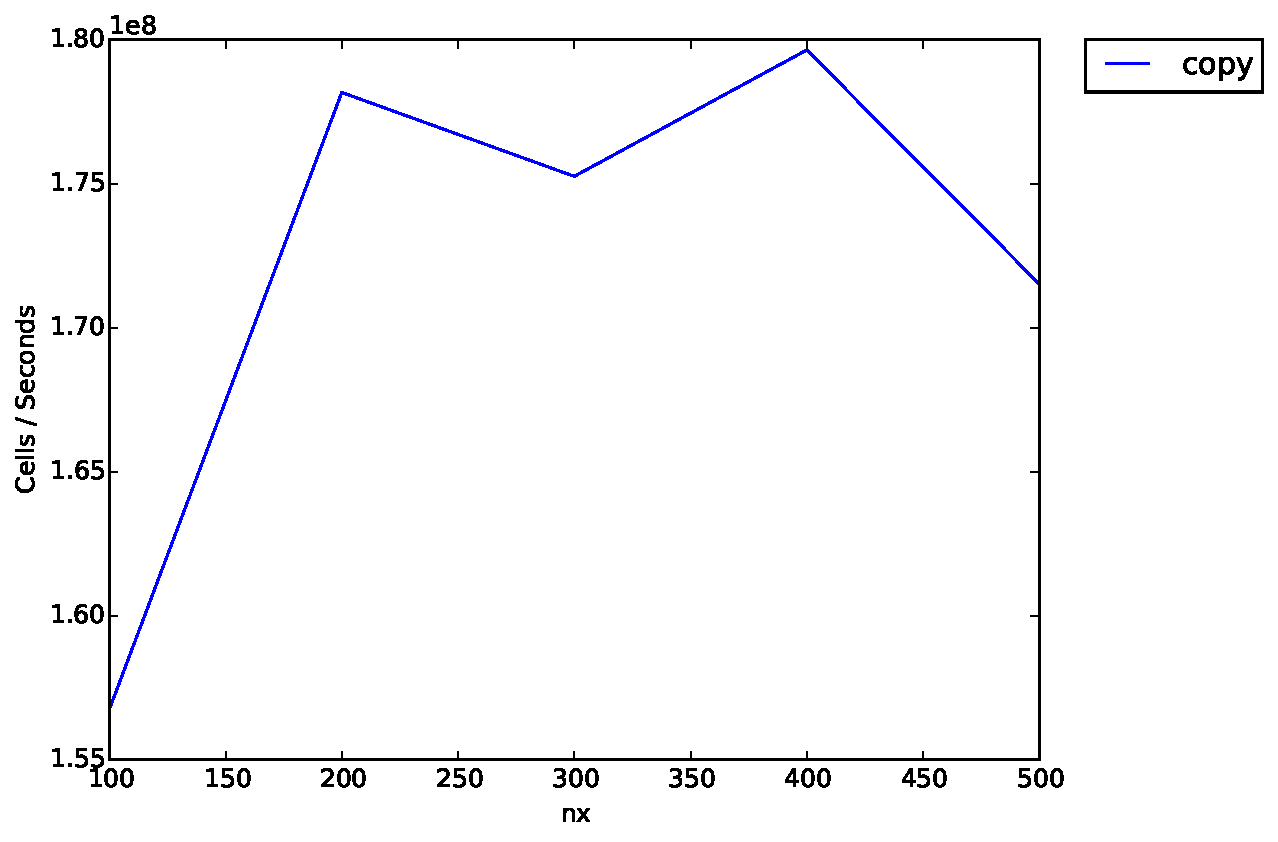
\includegraphics[width=0.8\textwidth]{figs/init-timing1.pdf}
    \caption{Initial Timing Result ($cells/seconds$ vs. $nx$)}
    \label{fig:initial_timing_result1}
\end{figure}

\begin{figure}[h]
    \centering
    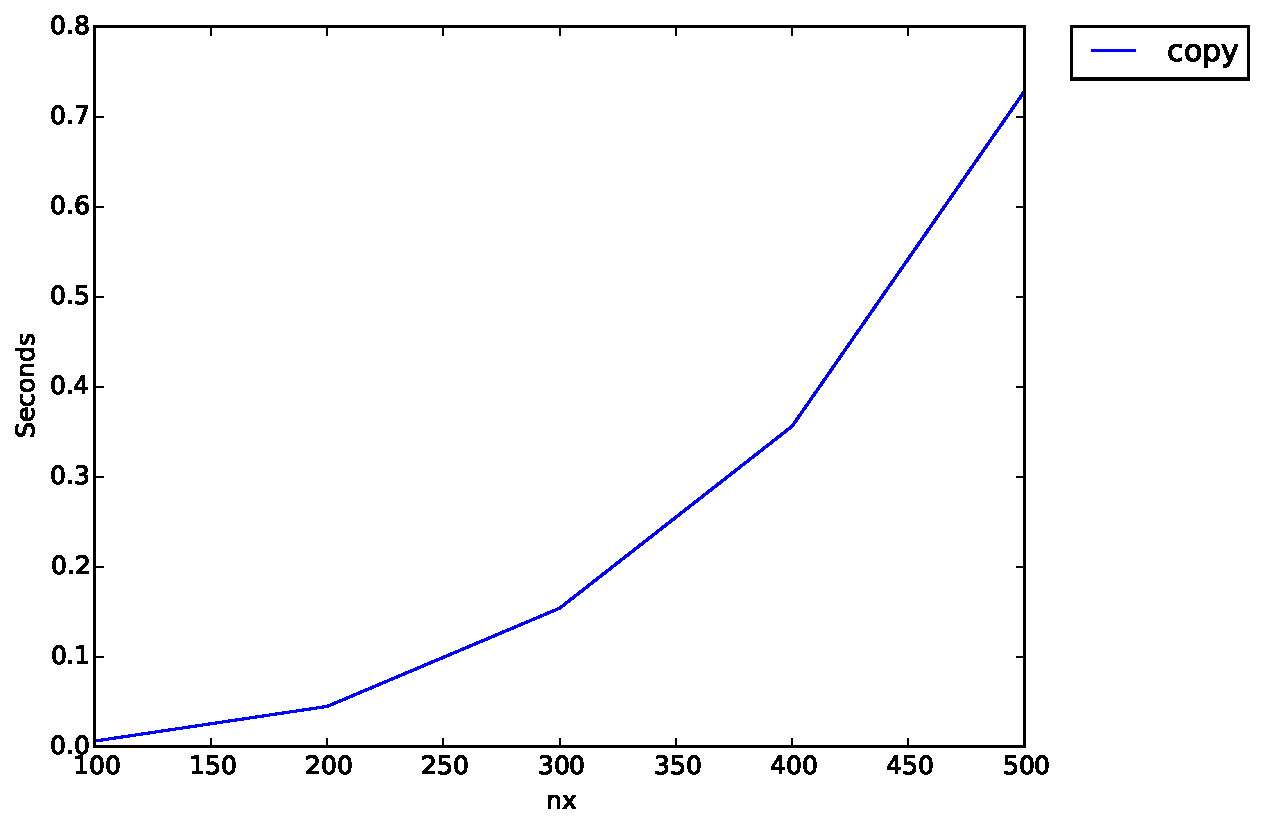
\includegraphics[width=0.8\textwidth]{figs/init-timing2.pdf}
    \caption{Initial Timing Result ($seconds$ vs. $nx$)}
    \label{fig:initial_timing_result2}
\end{figure}
